\section{CFG}

\frame{
	\frametitle{Context-free grammars}
	
	$G = \angbrack{\Sigma, N, S, R}$ \pause

	\begin{itemize}	
		\item	$\Sigma$ terminal vocabulary	\pause
		\item	$N$ nonterminal vocabulary \pause
		\item $S \in N$ start symbol \pause
		\item	$R \subseteq \{ A \rightarrow \alpha : A \in V, \alpha \in (\Sigma \cup V)^+  \}$ set of rules  
		
	\end{itemize}
	
}

\frame{
	\frametitle{CFG - example}
	
	Grammar \\
	\begin{columns}
		\begin{column}{0.5\textwidth}
			\begin{enumerate}
				\item $X \ra \text{a}$
				\item $X \ra \text{luz}$
				\item $X \ra \text{apague } X$
				\saveenum
			\end{enumerate}
		\end{column}
		\begin{column}{0.5\textwidth}
			\begin{enumerate}
				\resume
				\item $X \ra X \text{ por favor}$
				\item $X \ra X X$
				\item $S \ra X$
			\end{enumerate}
		\end{column}
	\end{columns}
	
	\pause
	
	~
	
	
	Discrete set
	\begin{itemize}
		\item infinite set of strings and trees
	\end{itemize}

}

\section{CKY}

\frame{
	\frametitle{Parsing a sentence}
	
	Input %\mxx
	\begin{itemize}
		\item sentence
	\end{itemize}
	\pause
	
	~
	
	Forest (analyses)
	\begin{itemize}
		\item subset of trees whose yield is the given sentence\\
		%$$S \ara{*} \mxx$$
	\end{itemize}
	\pause
	
	~
	
	CKY
	
	\begin{itemize}
		\item bottom-up dynamic program
	\end{itemize}
}

\frame[plain]{\frametitle{Parsing - example}
	
	\begin{footnotesize}
	\begin{tabular}{| c | p{1.55cm}  p{1.55cm}  p{1.55cm}  p{1.55cm}  p{1.55cm} |}
	\hline
	  & \multicolumn{1}{c}{\alert<5,7,12>{apague}} 
	  & \multicolumn{1}{c}{\alert<2>{a}} 
	  & \multicolumn{1}{c}{\alert<3>{luz}} 
	  & \multicolumn{1}{c}{\alert<6,9,13>{por}} 
	  & \multicolumn{1}{c|}{\alert<6,9,13>{favor}}  \\   \hline\hline 

	% ONE
	1 &        
	& \only<2->{\cellcolor{blue!10} $\alert<4,5,10>{X_{1,2}} \ara{1} \text{a}$}  
	& \only<3->{\cellcolor{blue!20} $\alert<4,6,8>{X_{2,3}} \ara{2} \text{luz}$} 
	& 
	& \\ \hline\hline
	
	% TWO
	\multirow{2}{*}{2} &        
	&  \multicolumn{2}{c}{ \only<4->{\cellcolor{green!10} $\alert<7,9>{X_{1,3}} \ara{5} X_{1,2} X_{2,3}$}} 
	& 
	& \\ %\cline{2-6}
	& \multicolumn{2}{c}{\only<5->{\cellcolor{green!20} $\alert<8,11>{X_{0,2}} \ara{3} \text{apague } X_{1,2}$}} 
	& \multicolumn{3}{c|}{\only<6->{\cellcolor{green!30} $\alert<10,11>{X_{2,5}} \ara{4} X_{2,3} \text{ por favor}$}} \\ \hline \hline
	 
	% THREE 
	  \multirow{4}{*}{3} 
	  & \multicolumn{3}{c}{\only<7->{\cellcolor{yellow!10} $\alert<13>{X_{0,3}} \ara{3} \text{apague } X_{1,3}$}} 
	  &  
	  & \\ %\cline{5-6}
	  & \multicolumn{3}{c}{\only<8->{\cellcolor{yellow!20} $X_{0,3} \ara{5} X_{0,2} X_{2,3}$}} 
	  &  
	  & \\ %\cline{2-6}
	  & 
	  & \multicolumn{4}{c|}{\only<9->{ \cellcolor{yellow!30} $\alert<12>{X_{1,5}} \ara{4} X_{1,3} \text{ por favor}$}} \\ %\cline{2-2}
	  & 
	  & \multicolumn{4}{c|}{\only<10->{\cellcolor{yellow!40} $X_{1,5} \ara{5} X_{1,2} X_{2,5}$}} \\ %\cline{2-6}
	  & \multicolumn{5}{c|}{\only<11->{\cellcolor{yellow!50}$X_{0,5} \ara{5} X_{0,2} X_{2,5} $}} \\ \hline \hline
	  
	  \multirow{2}{*}{4} 
	  & \multicolumn{5}{c|}{\only<12->{\cellcolor{orange!10} $\alert<14>{X_{0,5}} \ara{3} \text{apague } X_{1,5} $}} \\  
	  & \multicolumn{5}{c|}{\only<13->{\cellcolor{orange!20} $X_{0,5} \ara{4} X_{0,3} \text{ por favor} $}} \\ \hline \hline 
	   
	   5 & \multicolumn{5}{c|}{\only<14->{\cellcolor{red!10}$S_{0,5} \ara{6} X_{0,5}$}} \\ \hline   
	
	\end{tabular}
	\end{footnotesize}
	
	\begin{columns}
		\begin{column}{6cm}
			\begin{enumerate}
				\item \alert<2>{$X \ra \text{a}$}
				\item \alert<3>{$X \ra \text{luz}$}
				\item \alert<5,7,12>{$X \ra \text{apague } X$}
				\saveenum
			\end{enumerate}
		\end{column}
		\begin{column}{6cm}
			\begin{enumerate}
				\resume
				\item \alert<6,9,13>{$X \ra X \text{ por favor}$}
				\item \alert<4,8,10,11>{$X \ra X X$}
				\item \alert<14>{$S \ra X$}
			\end{enumerate}
		\end{column}
	\end{columns}
}

\frame{
	\frametitle{Forest}
	
	\begin{columns}
	
	\begin{column}{0.4\textwidth}\footnotesize
	\begin{enumerate}
		\item $X_{1,2} \ra \text{a}$
		\item $X_{2,3} \ra \text{luz}$

		\item $X_{0,2} \ra \text{apague } X_{1,2}$
		\item $X_{2,5} \ra X_{2,3} \text{ por favor}$
		\item $X_{1,3} \ra X_{1,2} X_{2,3}$
		
		\item $X_{1,5} \ra X_{1,2} X_{2,5}$
		\item $X_{0,3} \ra X_{0,2} X_{2,3}$
		\item $X_{0,5} \ra X_{0,2} X_{2,5}$
		\item $X_{0,3} \ra \text{apague } X_{1,3}$
		\item $X_{1,5} \ra X_{1,3} \text{ por favor}$
		
		\item $X_{0,5} \ra \text{apague } X_{1,5}$
		\item $X_{0,5} \ra X_{0,3} \text{ por favor}$
		
		\item $S_{0,5} \ra X_{0,5}$
	\end{enumerate}
	\end{column}
	
	\begin{column}{0.6\textwidth}
	\begin{itemize}
		\item<2-> the forest is itself a CFG
		\item<3-> nonterminals are annotated with input spans
		\item<4-> $O(n^2)$ specialised nonterminals
		\item<5-> $O(n^3)$ specialised rules
	\end{itemize}
	\end{column}
	
	\end{columns}
}

\frame{
	\frametitle{Hypergraph}
	
	A graphical representation for the forest
	\begin{itemize}
		\item<2-> (hyper)nodes represent (labelled) input spans
		\item<3-> (hyper)edges represent rules
		\begin{itemize}
			\item<4-> tail nodes: rule's \textsc{RHS}
			\item<5-> head node: rule's \textsc{LHS}
		\end{itemize}
	\end{itemize}
}

\frame{
	\frametitle{Analyses}
	
	Top-down traversals that rewrite every nonterminal \pause
	
	\scalebox{0.65}{
	\Tree [.$S_{0,5}$ 
			[.$X_{0,3}$ 
				{apague}
				[.$X_{1,3}$ 
					[.$X_{1,2}$ a ]
					[.$X_{2,3}$ luz ]
				]
			] 
			{por favor}
		]		
	}\pause
	\scalebox{0.65}{
	\Tree [.$S_{0,5}$ 
			[.$X_{0,5}$ 
				{apague}
				[.$X_{1,5}$ 
					[.$X_{1,3}$
						[.$X_{1,2}$ a ]
						[.$X_{1,2}$ luz ]
					]
					{por favor}
				]
			] 
		]
	}\pause
	\scalebox{0.65}{
	\Tree [.$S_{0,5}$ 
			[.$X_{0,5}$ 
				[.$X_{0,2}$ 
					{apague}
					[.$X_{1,2}$ a ]
				]
				[.$X_{2,5}$ 
					[.$X_{2,3}$ luz ]
					{por favor}
				]
			] ]		
	}	
	
}

\section{Parsing as intersection}

\frame{
	\frametitle{Parsing as intersection}
	
	Input
	\begin{itemize}
		\item linear-chain finite-state automaton
	\end{itemize}
	
	\scalebox{0.6}{	
	\begin{tikzpicture}[->,>=stealth',shorten >=1pt,auto,node distance=2.8cm,semithick]
  	\tikzstyle{every state}=[draw=black,text=black]
	  	\node[initial,state,style={initial text=}] (A) {$0$};
		\node[state] (B) [right of=A] {$1$};
		\node[state] (C) [right of=B] {$2$};
		\node[state] (D) [right of=C] {$3$};
		\node[state] (E) [right of=D] {$4$};
		\node[state,accepting] [right of=E] (F) {$5$};

		\path[color=black] 
			(A) edge node {apague} (B)
			(B) edge node {a} (C)
			(C) edge node {luz} (D)
			(D) edge node {por} (E)
			(E) edge node {favor} (F);
	
	\end{tikzpicture} 
	}

	~
	
	Output
	\begin{itemize}
		\item subset of parse trees yielding valid input strings  
	\end{itemize}
		
}

\frame{
	\frametitle{Finite-state automata}
	
	$G = \angbrack{\Sigma, Q, I, F, E}$ \pause
	
	\begin{itemize}	
		\item	$\Sigma$ terminal vocabulary	\pause
		\item	$Q$ set of states \pause
		\item $I \subseteq Q$ set of initial states \pause
		\item $F \subseteq Q$ set of final states \pause 
		\item	$E \subseteq Q \times \Sigma \times Q$ is a set of labelled transitions \pause
		\item $\angbrack{q, x, s} \in E$ where $q \in Q$, $s \in Q$ and $x \in \Sigma$ \\
		is a transition from $q$ to $s$ which recognises $x$
	\end{itemize}
}

\frame{
	\frametitle{Deductive proof system}

	A proof starts from its \textsc{Axioms}
	$$\drule{}{\textcolor{blue}{\itembrack{\textsc{axiom}}}}{\alert{\text{predicate}}}$$
	
	\hfill where \itembrack{\textsc{axiom}} is an item

	\pause
	
	
	and it follows by {\bf exhaustive} deduction of new items
	$$\drule{\textcolor{Green}{\itembrack{\alpha_1} \itembrack{\alpha_2}} \ldots \textcolor{Green}{\itembrack{\alpha_n}}}{\textcolor{blue}{\itembrack{\alpha_{n+1}}}}{\alert{\text{predicate}}}$$
	\begin{itemize}
		\item \textcolor{Green}{antecedents}
		\item \textcolor{blue}{consequent}
		\item \alert{conditions}
	\end{itemize}
	
	\pause
	
	the proof is valid if a {\bf goal item} is provable
	
}


\frame{
	\frametitle{Bottom-up parsing}

	\begin{columns}
	
	\begin{column}{7cm}\footnotesize
	\begin{align*}
	\textsc{Axioms} & \\
	& \drule{}{\itembrack{X \ra \bullet \alpha, q, q}}{q \in Q \wedge X \ra \alpha \in R} \\
	\textsc{Goal} & \\
	& \itembrack{S \ra \alpha \bullet, q, r} ~ q \in I \wedge r \in F\\
	\textsc{Scan} & \\
	& \drule{\itembrack{X \ra \alpha \bullet x \beta, q, s}}{\itembrack{X \ra \alpha x \bullet \beta}}{\angbrack{s, x, r} \in E}\\
	\textsc{Complete} & \\
	& \drule{\itembrack{X \ra \alpha \bullet Y \beta, q, s}\itembrack{Y \ra \gamma \bullet, s, r}}{\itembrack{X \ra \alpha Y_{s,r} \bullet \beta, q, r}}{}
	\end{align*}
	\end{column}
	
	\begin{column}{7cm}
		\begin{itemize}
			\item self-contained ``algorithm''
			\item template for a hypergraph
		\end{itemize}
	\end{column}

	\end{columns}
	

}


\frame[plain]{
	\frametitle{Axioms}
	\begin{enumerate}
		\item \itembrack{X \ra \bullet \text{a}, 1, 1} \pause
		\item \itembrack{X \ra \bullet \text{luz}, 2, 2} \pause
		\item \itembrack{X \ra \bullet \text{apague } X, 0, 0} \pause
		\item \itembrack{X \ra \bullet X \text{ por favor}, 0, 0} \pause
	 	\item \itembrack{X \ra \bullet X \text{ por favor}, 1, 1} \pause
	 	\item \itembrack{X \ra \bullet X \text{ por favor}, 2, 2} \pause
	 	\item \itembrack{X \ra \bullet X X, 0, 0} \pause
	    \item \itembrack{X \ra \bullet X X, 1, 1} \pause
	    \item \itembrack{X \ra \bullet X X, 2, 2} \pause
	    \item \itembrack{X \ra \bullet X X, 3, 3} \pause
	 	\item \itembrack{S \ra \bullet X, 0, 0}
	\end{enumerate}
}




\frame[plain]{
	\frametitle{Inference}
	
	\begin{columns}[T]
	\begin{column}{6.5cm}
	
	\begin{enumerate}\footnotesize
		\item \only<1>{\itembrack{X \ra \bullet \alert{\text{a}}, 1, \alert{1}}\textcolor{red}{\la}}\only<2-22>{\itembrack{X \ra \textcolor{Green}{\text{a}} \bullet, 1, 2} \textcolor{Green}{scanned}}\only<23>{\itembrack{X \ra \textcolor{Green}{\text{a}} \bullet, 1, 2} \alert{\la}}\only<24->{\itembrack{X \ra \textcolor{Green}{\text{a}} \bullet, 1, 2} \textcolor{blue}{$\checkmark$}}
		\item \only<1>{\itembrack{X \ra \bullet \text{luz}, 2, 2}}\only<2>{\itembrack{X \ra \bullet \alert{\text{luz}}, 2, \alert{2}}\textcolor{red}{\la}}\only<3-23>{\itembrack{X \ra \textcolor{Green}{\text{luz}}\bullet, 2, 3} \textcolor{Green}{scanned}}\only<24>{\itembrack{X \ra \textcolor{Green}{\text{luz}}\bullet, 2, 3} \alert{\la}}\only<25->{\itembrack{X \ra \textcolor{Green}{\text{luz}}\bullet, 2, 3} \textcolor{blue}{$\checkmark$}}
		\item \only<1-2>{\itembrack{X \ra \bullet \text{apague} X, 0, 0}}\only<3>{\itembrack{X \ra \bullet \alert{\text{apague}} X, 0, \alert{0}}\textcolor{red}{\la}}\only<4-24>{\itembrack{X \ra \textcolor{Green}{\text{apague}} \bullet X, 0, 1} \textcolor{Green}{scanned}}\only<25-28>{\itembrack{X \ra \textcolor{Green}{\text{apague}} \bullet \alert{X}, 0, \alert{1}} \alert{\la}}\only<29->{\itembrack{X \ra \textcolor{Green}{\text{apague}} \bullet \textcolor{Orange}{X}, 0, \textcolor{Orange}{1}} \textcolor{Orange}{waiting}}
	 	\item \only<1-3>{\itembrack{X \ra \bullet X \text{ por favor}, 1, 1}}\only<4-5>{\itembrack{X \ra \bullet \alert{X} \text{ por favor}, 1, \alert{1}}\textcolor{red}{\la}}\only<6-28,31->{\itembrack{X \ra \bullet \textcolor{Orange}{X} \text{ por favor}, 1, \textcolor{Orange}{1}} \textcolor{Orange}{waiting}}\only<29-30>{\itembrack{X \ra \bullet \alert{X} \text{ por favor}, 1, \alert{1}} \alert{\la}}
	 	\item \only<1-5>{\itembrack{X \ra \bullet X \text{ por favor}, 2, 2}}\only<6-7,31>{\itembrack{X \ra \bullet \alert{X} \text{ por favor}, 2, \alert{2}}\alert{\la}}\only<8-30>{\itembrack{X \ra \bullet \textcolor{Orange}{X} \text{ por favor}, 2, \textcolor{Orange}{2}} \textcolor{Orange}{waiting}}\only<32->{\itembrack{X \ra \bullet \textcolor{Orange}{X} \text{ por favor}, 2, \textcolor{Orange}{2}} \textcolor{Orange}{waiting}}
	 	\item \only<1-7>{\itembrack{X \ra \bullet X X, 0, 0}}\only<8,32-34>{\itembrack{X \ra \bullet \alert{X} X, 0, \alert{0}}\alert{\la}}\only<9-31,35->{\itembrack{X \ra \bullet \textcolor{Orange}{X} X, 0, \textcolor{Orange}{0}} \textcolor{Orange}{waiting}}
	    \item \only<1-8>{\itembrack{X \ra \bullet X X, 1, 1}}\only<9-10,35-36>{\itembrack{X \ra \bullet \alert{X} X, 1, \alert{1}} \alert{\la}}\only<11-34,37->{\itembrack{X \ra \bullet \textcolor{Orange}{X} X, 1, \textcolor{Orange}{1}}  \textcolor{Orange}{waiting}}
	    \item \only<1-10>{\itembrack{X \ra \bullet X X, 2, 2}}\only<11-12,37>{\itembrack{X \ra \bullet \alert{X} X, 2, \alert{2}}\alert{\la}}\only<13-36,38->{\itembrack{X \ra \bullet \textcolor{Orange}{X} X, 2, \textcolor{Orange}{2}} \textcolor{Orange}{waiting}}
	    \item \only<1-12>{\itembrack{X \ra \bullet X X, 3, 3}}\only<13,38>{\itembrack{X \ra \bullet \alert{X} X, 3, \alert{3}}\alert{\la}}\only<14-37,39->{\itembrack{X \ra \bullet \textcolor{Orange}{X} X, 3, \textcolor{Orange}{3}} \textcolor{Orange}{waiting}}
	 	\item \only<1-13>{\itembrack{S \ra \bullet X, 0, 0}}\only<14,39-40>{\itembrack{S \ra \bullet \alert{X}, 0, \alert{0}}\alert{\la}}\only<15-38,41->{\itembrack{S \ra \bullet \textcolor{Orange}{X}, 0, \textcolor{Orange}{0}} \textcolor{Orange}{waiting}}%%%%
		\only<5-14>{\item \itembrack{X \ra \textcolor{blue}{X_{1,2}} \bullet \text{ por favor}, 1, 2} \textcolor{blue}{completed}}\only<15>{\item \itembrack{X \ra \textcolor{blue}{X_{1,2}} \bullet \alert{\text{por favor}}, 1, \alert{2}} \alert{\la}}\only<16->{\textcolor{gray}{\item \itembrack{X \ra X_{1,2} \bullet \text{por favor}, 1, 2} $\times$}}
		\only<7-15>{\item \itembrack{X \ra \textcolor{blue}{X_{2,3}} \bullet \text{ por favor}, 2, 3} \textcolor{blue}{completed}}\only<16>{\item \itembrack{X \ra \textcolor{blue}{X_{2,3}} \bullet \alert{\text{ por favor}}, 2, \alert{3}} \alert{\la}}\only<17-40>{\item \itembrack{X \ra \textcolor{blue}{X_{2,3}} \textcolor{Green}{\text{ por favor}} \bullet, 2, 5} \textcolor{Green}{scanned}}\only<41>{\item \itembrack{X \ra \textcolor{blue}{X_{2,3}} \textcolor{Green}{\text{ por favor}} \bullet, 2, 5} \alert{\la}}\only<42->{\item \itembrack{X \ra \textcolor{blue}{X_{2,3}} \textcolor{Green}{\text{ por favor}} \bullet, 2, 5} \textcolor{blue}{$\checkmark$}}
		\only<10-16>{\item \itembrack{X \ra \textcolor{blue}{X_{1,2}} \bullet X, 1, 2} \textcolor{blue}{completed}}\only<17-19,42>{\item \itembrack{X \ra \textcolor{blue}{X_{1,2}} \bullet \alert{X}, 1, \alert{2}} \alert{\la}}\only<20-41,43->{\item \itembrack{X \ra \textcolor{blue}{X_{1,2}} \bullet \textcolor{Orange}{X}, 1, \textcolor{Orange}{2}} \textcolor{Orange}{waiting}}
		\only<12-19>{\item \itembrack{X \ra \textcolor{blue}{X_{2,3}} \bullet X, 2, 3} \textcolor{blue}{completed}}\only<20,43>{\item \itembrack{X \ra \textcolor{blue}{X_{2,3}} \bullet \alert{X}, 2, \alert{3}} \alert{\la}}\only<21-42,44->{\item \itembrack{X \ra \textcolor{blue}{X_{2,3}} \bullet \textcolor{Orange}{X}, 2, \textcolor{Orange}{3}} \textcolor{Orange}{waiting}}
		\only<18-20>{\item \itembrack{X \ra \textcolor{blue}{X_{1,2} X_{2,3}} \bullet , 1, 3} \textcolor{blue}{completed}}\only<21>{\item \itembrack{X \ra \textcolor{blue}{X_{1,2} X_{2,3}} \bullet , 1, 3} \alert{\la}}\only<22->{\item \itembrack{X \ra \textcolor{blue}{X_{1,2} X_{2,3}} \bullet , 1, 3} \textcolor{blue}{$\checkmark$}}
		\only<19-21>{\item \itembrack{X \ra \textcolor{blue}{X_{1,2} X_{2,5}} \bullet , 1, 5} \textcolor{blue}{completed}}\only<22>{\item \itembrack{X \ra \textcolor{blue}{X_{1,2} X_{2,5}} \bullet , 1, 5} \alert{\la}}\only<23->{\item \itembrack{X \ra \textcolor{blue}{X_{1,2} X_{2,5}} \bullet , 1, 5} \textcolor{blue}{$\checkmark$}}
		\saveenum
	\end{enumerate}
	\end{column}

	\begin{column}{7cm}

	\only<26->{
	\begin{enumerate}\footnotesize\resume
		\only<26-43>{\item \itembrack{X \ra \textcolor{Green}{\text{apague }} \textcolor{blue}{X_{1,2}} \bullet , 0, 2} \textcolor{blue}{completed}}\only<44>{\item \itembrack{X \ra \textcolor{Green}{\text{apague }} \textcolor{blue}{X_{1,2}} \bullet , 0, 2} \alert{\la}}\only<45->{\item \itembrack{X \ra \textcolor{Green}{\text{apague }} \textcolor{blue}{X_{1,2}} \bullet , 0, 2} \textcolor{blue}{$\checkmark$}}
		\only<27-44>{\item \itembrack{X \ra \textcolor{Green}{\text{apague }} \textcolor{blue}{X_{1,3}} \bullet , 0, 3} \textcolor{blue}{completed}}\only<45>{\item \itembrack{X \ra \textcolor{Green}{\text{apague }} \textcolor{blue}{X_{1,3}} \bullet , 0, 3} \alert{\la}}\only<46->{\item \itembrack{X \ra \textcolor{Green}{\text{apague }} \textcolor{blue}{X_{1,3}} \bullet , 0, 3} \textcolor{blue}{$\checkmark$}}
		\only<28-45>{\item \itembrack{X \ra \textcolor{Green}{\text{apague }} \textcolor{blue}{X_{1,5}} \bullet , 0, 5} \textcolor{blue}{completed}}\only<46>{\item \itembrack{X \ra \textcolor{Green}{\text{apague }} \textcolor{blue}{X_{1,5}} \bullet , 0, 5} \alert{\la}}\only<47->{\item \itembrack{X \ra \textcolor{Green}{\text{apague }} \textcolor{blue}{X_{1,5}} \bullet , 0, 5} \textcolor{blue}{$\checkmark$}}
		\only<30-46>{\item \itembrack{X \ra \textcolor{blue}{X_{1,3}} \bullet \text{ por favor}, 1, 3}  \textcolor{blue}{completed}}\only<47>{\item \itembrack{X \ra \textcolor{blue}{X_{1,3}} \bullet \alert{\text{ por favor}}, 1, \alert{3}}  \alert{\la}}\only<48-65>{\item \itembrack{X \ra \textcolor{blue}{X_{1,3}} \textcolor{Green}{\text{ por favor}} \bullet, 1, 5}  \textcolor{Green}{scanned}}\only<66>{\item \itembrack{X \ra \textcolor{blue}{X_{1,3}} \textcolor{Green}{\text{ por favor}} \bullet, 1, 5}  \alert{\la}}
		\only<67->{\item \itembrack{X \ra \textcolor{blue}{X_{1,3}} \textcolor{Green}{\text{ por favor}} \bullet, 1, 5}  \textcolor{blue}{$\checkmark$}}
		\only<33-47>{\item \itembrack{X \ra \textcolor{blue}{X_{0,2}} \bullet X, 0, 2} \textcolor{blue}{completed}}\only<48-50>{\item \itembrack{X \ra \textcolor{blue}{X_{0,2}} \bullet \alert{X}, 0, \alert{2}} \alert{\la}}\only<51->{\item \itembrack{X \ra \textcolor{blue}{X_{0,2}} \bullet \textcolor{Orange}{X}, 0, \textcolor{Orange}{2}} \textcolor{Orange}{waiting}}
		\only<34-50>{\item \itembrack{X \ra \textcolor{blue}{X_{0,3}} \bullet X, 0, 3} \textcolor{blue}{completed}}\only<51>{\item \itembrack{X \ra \textcolor{blue}{X_{0,3}} \bullet \alert{X}, 0, \alert{3}} \alert{\la}}\only<52->{\item \itembrack{X \ra \textcolor{blue}{X_{0,3}} \bullet \textcolor{Orange}{X}, 0, \textcolor{Orange}{3}} \textcolor{Orange}{waiting}}
		\only<36-51>{\item \itembrack{X \ra \textcolor{blue}{X_{1,3}} \bullet X, 1, 3} \textcolor{blue}{completed}}\only<52>{\item \itembrack{X \ra \textcolor{blue}{X_{1,3}} \bullet \alert{X}, 1, \alert{3}} \alert{\la}}\only<53->{\item \itembrack{X \ra \textcolor{blue}{X_{1,3}} \bullet \textcolor{Orange}{X}, 1, \textcolor{Orange}{3}} \textcolor{Orange}{waiting}}
		\only<40-52>{\item \itembrack{S \ra \textcolor{blue}{X_{0,5}} \bullet, 0, 5} \textcolor{blue}{completed}}\only<53>{\item \itembrack{S \ra \textcolor{blue}{X_{0,5}} \bullet, 0, 5} \alert{\la}}\only<54->{\item \itembrack{S \ra \textcolor{blue}{X_{0,5}} \bullet, 0, 5} \textcolor{blue}{$\checkmark$}}
		\only<49-53>{\item \itembrack{X \ra \textcolor{blue}{X_{0,2}} \textcolor{blue}{X_{2,3}} \bullet, 0, 3} \textcolor{blue}{completed}}\only<54>{\item \itembrack{X \ra \textcolor{blue}{X_{0,2}} \textcolor{blue}{X_{2,3}} \bullet, 0, 3} \alert{\la}}\only<55->{\item \itembrack{X \ra \textcolor{blue}{X_{0,2}} \textcolor{blue}{X_{2,3}} \bullet, 0, 3} \textcolor{blue}{$\checkmark$}}
		\only<50-54>{\item \itembrack{X \ra \textcolor{blue}{X_{0,2}} \textcolor{blue}{X_{2,5}} \bullet, 0, 5} \textcolor{blue}{completed}}\only<55>{\item \itembrack{X \ra \textcolor{blue}{X_{0,2}} \textcolor{blue}{X_{2,5}} \bullet, 0, 5} \alert{\la}}\only<56->{\item \itembrack{X \ra \textcolor{blue}{X_{0,2}} \textcolor{blue}{X_{2,5}} \bullet, 0, 5} \textcolor{blue}{$\checkmark$}}
		\only<57>{\item \itembrack{X \ra \bullet X \text{ por favor}, 0, 0}}
		\only<58-61>{\item \itembrack{X \ra \bullet \alert{X} \text{ por favor}, 0, \alert{0}} \alert{\la}}
		\only<62->{\item \itembrack{X \ra \bullet \textcolor{Orange}{X} \text{ por favor}, 0, \textcolor{Orange}{0}} \textcolor{Orange}{waiting}}
		\only<59-61>{\item \itembrack{X \ra \textcolor{blue}{X_{0,2}} \bullet \text{ por favor}, 0, 2} \textcolor{blue}{completed}}
		\only<62>{\item \itembrack{X \ra \textcolor{blue}{X_{0,2}} \bullet \alert{\text{ por favor}}, 0, \alert{2}} \alert{\la}}
		\textcolor{gray}{\only<63->{\item \itembrack{X \ra X_{0,2} \bullet \text{ por favor}, 0, 2}  $\times$}}
		\only<60-62>{\item \itembrack{X \ra \textcolor{blue}{X_{0,3}} \bullet \text{ por favor}, 0, 3} \textcolor{blue}{completed}}
		\only<63>{\item \itembrack{X \ra \textcolor{blue}{X_{0,3}} \bullet \alert{\text{ por favor}}, 0, \alert{3}} \alert{\la}}
		\only<64-67>{\item \itembrack{X \ra \textcolor{blue}{X_{0,3}} \textcolor{Green}{\text{ por favor}} \bullet, 0, 5} \textcolor{Green}{scanned}}
		\only<68>{\item \itembrack{X \ra \textcolor{blue}{X_{0,3}} \textcolor{Green}{\text{ por favor}} \bullet, 0, 5} \alert{\la}}
		\only<69>{\item \itembrack{X \ra \textcolor{blue}{X_{0,3}} \textcolor{Green}{\text{ por favor}} \bullet, 0, 5} \textcolor{blue}{$\checkmark$}}
		\only<61-63>{\item \itembrack{X \ra \textcolor{blue}{X_{0,5}} \bullet \text{ por favor}, 0, 5} \textcolor{blue}{completed}}
		\only<64>{\only<61->{\item \itembrack{X \ra \textcolor{blue}{X_{0,5}} \bullet \alert{\text{ por favor}}, 0, \alert{5}} \alert{\la}}}
		\textcolor{gray}{\only<65->{\item \itembrack{X \ra X_{0,5} \bullet \text{ por favor}, 0, 5} $\times$}}		
	\end{enumerate}
	}

	\end{column}
	

	
	\end{columns}

}

\frame{
	\frametitle{Forest}
	
	\begin{enumerate}
		\item \itembrack{X_{1,2} \ra \text{a}}
		\item \itembrack{X_{2,3} \ra \text{luz}}
		
		\item \itembrack{X_{0,2} \ra \text{apague } X_{1,2}}
		\item \itembrack{X_{2,5} \ra X_{2,3} \text{ por favor}}
		\item \itembrack{X_{1,3} \ra X_{1,2} X_{2,3}}
		
		\item \itembrack{X_{1,5} \ra X_{1,2} X_{2,5}}
		\item \itembrack{X_{0,3} \ra X_{0,2} X_{2,3}}
		\item \itembrack{X_{0,5} \ra X_{0,2} X_{2,5}}
		\item \itembrack{X_{0,3} \ra \text{apague } X_{1,3}}
		\item \itembrack{X_{1,5} \ra X_{1,3} \text{ por favor}}

		\item \itembrack{X_{0,5} \ra \text{apague } X_{1,5}}
		\item \itembrack{X_{0,5} \ra X_{0,3} \text{ por favor}}

		\item \itembrack{S_{0,5} \ra X_{0,5}}

	\end{enumerate}
}



\section{SCFG}

\frame{
	\frametitle{Synchronous context-free grammars}
	
	$G = \angbrack{\Sigma, \Delta, N, S, R}$ \pause

	\begin{itemize}	
		\item	$\Sigma$ input terminal vocabulary	\pause
		\item	$\Delta$ output terminal vocabulary	\pause
		\item	$N$ shared nonterminal vocabulary \pause
		\item $S \in N$ start symbol \pause
		\item $R$ is a set of synchronous rules\\ \pause
		each of the form $X \ra \angbrack{\alpha, \beta, \sim}$ \pause
		\begin{itemize}
			\item $X \in N$ \pause
			\item $\alpha \in (\Sigma \cup N)^+$ \pause
			\item $\beta \in (\Delta \cup N)^+$ \pause
			\item $\sim$ is a one-to-one mapping between nonterminals in $\alpha$ and $\beta$
		\end{itemize}
		
		%\item	$R \subseteq \{ A \rightarrow \alpha : A \in V, \alpha \in (\Sigma \cup V)^+  \}$ set of rules
%		\item $\omega: R \rightarrow \Reals$ is a function that assigns weights to rules \\
	\end{itemize}
}

\frame{
	\frametitle{SCFG - example}
	
	Synchronous grammar \\
			\begin{enumerate}
				\item $X \ra \angbrack{\ftext{a}, \etext{the}}$
				\item $X \ra \angbrack{\ftext{luz}, \etext{light}}$
				\item $X \ra \angbrack{\ftext{apague } X_1, \etext{switch } X_1 \etext{ off}}$
				\item $X \ra \angbrack{X_1 \ftext{ por favor}, \etext{please, } X_1}$
				\item $X \ra \angbrack{X_1 X_2, X_1 X_2}$
				\item $S \ra \angbrack{X_1, X_1}$
			\end{enumerate}

}

\section{Synchronous parsing}

\frame{
	\frametitle{Synchronous parsing}

	Recognise pair of strings \pause
	
	~
	
	Example
	
	$$\angbrack{\ftext{apague a luz por favor}, \etext{please, switch off the light}}$$
	
	~\pause
	
	A valid tree yields a pair of strings
		
	
}

\frame{
	\frametitle{Two intersections}
	
	Intersect the input
	\begin{enumerate}
		\pause
		\item a valid tree yields the input string \pause
		\item the intersection itself is a CFG \pause
		\item an output projection defines a set of output strings \pause
	\end{enumerate}
	
	Intersect the output \pause
	\begin{enumerate}
		\item a valid tree yields the output string
	\end{enumerate}
}

\frame{
	\frametitle{CKY+}
	
	\begin{columns}
	
	\begin{column}{6cm}\footnotesize
	\begin{align*}
	\textsc{Axioms} & \\
	& \drule{}{\itembrack{X \ra \angbrack{\bullet \beta, \zeta}, q, q}}{q \in Q \wedge X \ra \angbrack{\beta, \zeta} \in R} \\
	\textsc{Goal} & \\
	& \itembrack{X \ra \angbrack{\alpha \bullet, \zeta}, q, r} ~ q \in I \wedge r \in F \wedge X \in S\\
	\textsc{Scan} & \\
	& \drule{\itembrack{X \ra \angbrack{\alpha \bullet x \beta, \zeta}, q, s}}{\itembrack{X \ra \angbrack{\alpha x \bullet \beta, \zeta}}}{\angbrack{s, x, r} \in E}\\
	\textsc{Complete} & \\
	& \drule{\itembrack{X \ra \angbrack{\alpha \bullet Y \beta, \zeta}, q, s}\itembrack{Y \ra \angbrack{\gamma \bullet, \xi}, s, r}}{\itembrack{X \ra \angbrack{\alpha Y_{s,r} \bullet \beta, \zeta}, q, r}}{}
	\end{align*}
	\end{column}
	
	\begin{column}{4cm}
	\begin{itemize}
		\item algorithm remains the same
		\item keep track of target \textsc{RHS}
	\end{itemize}
	\end{column}
	\end{columns}
}


\frame{
	\frametitle{First intersection}
	
	\begin{columns}
	
	\begin{column}{0.7\textwidth}\footnotesize
	\begin{enumerate}
		\item $X_{1,2} \ra \angbrack{\ftext{a}, \etext{the}}$
		\item $X_{2,3} \ra \angbrack{\ftext{luz}, \etext{light}}$

		\item $X_{0,2} \ra \angbrack{\ftext{apague } X_{1,2}, \etext{switch } X_{1,2} \etext{ off}}$
		\item $X_{2,5} \ra \angbrack{X_{2,3} \ftext{ por favor}, \etext{please, } X_{2,3}}$
		\item $X_{1,3} \ra \angbrack{X_{1,2} X_{2,3}, X_{1,2} X_{2,3}}$
		
		\item $X_{1,5} \ra \angbrack{X_{1,2} X_{2,5}, X_{1,2} X_{2,5}}$
		\item $X_{0,3} \ra \angbrack{X_{0,2} X_{2,3}, X_{0,2} X_{2,3}}$
		\item $X_{0,5} \ra \angbrack{X_{0,2} X_{2,5}, X_{0,2} X_{2,5}}$
		\item $X_{0,3} \ra \angbrack{\ftext{apague } X_{1,3}, \etext{switch } X_{1,3} \etext{ off}}$
		\item $X_{1,5} \ra \angbrack{X_{1,3} \ftext{ por favor}, \etext{please, } X_{1,3}}$
		
		\item $X_{0,5} \ra \angbrack{\ftext{apague } X_{1,5}, \etext{switch } X_{1,5} \etext{ off}}$
		\item $X_{0,5} \ra \angbrack{X_{0,3} \ftext{ por favor}, \etext{please, } X_{0,3}}$
		
		\item $S_{0,5} \ra \angbrack{X_{0,5}, X_{0,5}}$
	\end{enumerate}
	\end{column}
	\end{columns}
}


\frame{
	\frametitle{Projection}
	
	\begin{columns}
	
	\begin{column}{0.7\textwidth}\footnotesize
	\only<1>{
	\begin{enumerate}
		\item $X_{1,2} \ra \etext{the}$
		\item $X_{2,3} \ra \etext{light}$

		\item $X_{0,2} \ra \etext{switch } X_{1,2} \etext{ off}$
		\item $X_{2,5} \ra \etext{please, } X_{2,3}$
		\item $X_{1,3} \ra X_{1,2} X_{2,3}$
		
		\item $X_{1,5} \ra X_{1,2} X_{2,5}$
		\item $X_{0,3} \ra X_{0,2} X_{2,3}$
		\item $X_{0,5} \ra X_{0,2} X_{2,5}$
		\item $X_{0,3} \ra \etext{switch } X_{1,3} \etext{ off}$
		\item $X_{1,5} \ra \etext{please, } X_{1,3}$
		
		\item $X_{0,5} \ra \etext{switch } X_{1,5} \etext{ off}$
		\item $X_{0,5} \ra \etext{please, } X_{0,3}$
		
		\item $S_{0,5} \ra X_{0,5}$
	\end{enumerate}
	}
	\only<2>{
	\begin{enumerate}
		\item $X^{1,2} \ra \etext{the}$
		\item $X^{2,3} \ra \etext{light}$

		\item $X^{0,2} \ra \etext{switch } X^{1,2} \etext{ off}$
		\item $X^{2,5} \ra \etext{please, } X^{2,3}$
		\item $X^{1,3} \ra X^{1,2} X^{2,3}$
		
		\item $X^{1,5} \ra X^{1,2} X^{2,5}$
		\item $X^{0,3} \ra X^{0,2} X^{2,3}$
		\item $X^{0,5} \ra X^{0,2} X^{2,5}$
		\item $X^{0,3} \ra \etext{switch } X^{1,3} \etext{ off}$
		\item $X^{1,5} \ra \etext{please, } X^{1,3}$
		
		\item $X^{0,5} \ra \etext{switch } X^{1,5} \etext{ off}$
		\item $X^{0,5} \ra \etext{please, } X^{0,3}$
		
		\item $S^{0,5} \ra X^{0,5}$
	\end{enumerate}
	}
	\end{column}
	\end{columns}
}

\frame[plain]{
	\frametitle{Second intersection}
	
	
	\footnotesize
	
	\begin{tabular}{| l | p{1.5cm}  p{1.5cm} p{1.5cm}  p{1.5cm} p{1.5cm} |}
	\hline
	  & please, & switch & the & light & off \\ \hline\hline
	1 & 
	& 
	& \multicolumn{1}{c}{\only<2->{\cellcolor{blue!10} $X^{1,2}_{\only<8->{\textcolor{blue}{2,3}}} \ara{1} \text{the}$}} 
	& \multicolumn{1}{c}{\only<3->{\cellcolor{blue!20} $X^{2,3}_{\only<9->{\textcolor{blue}{3,4}}} \ara{2} \text{light}$}}  
	& \\ \hline\hline
	
	2 & 
	& 
	& \multicolumn{2}{c}{\only<4->{\cellcolor{green!10} $X^{1,3}_{\only<10->{\textcolor{blue}{2,4}}} \ara{5} X^{1,2}_{\only<11->{\textcolor{blue}{2,3}}} X^{2,3}_{\only<12->{\textcolor{blue}{3,4}}}$}}
	 
	& \\ \hline\hline
	
	3 &  
	& \multicolumn{4}{c|}{\only<5->{\cellcolor{yellow!10} $X^{0,3}_{\only<13->{\textcolor{blue}{1,5}}} \ara{9} \text{switch } X^{1,3}_{\only<14->{\textcolor{blue}{2,4}}} \text{ off}$}}
	 
	 \\ \hline\hline
	 
	4 &  
	 \multicolumn{5}{c|}{\only<6->{\cellcolor{orange!10} $X^{0,5}_{\only<15->{\textcolor{blue}{0,5}}} \ara{12} \text{please,} X^{0,3}_{\only<16->{\textcolor{blue}{1,5}}}$}}
	 
	 \\ \hline\hline
	 
	 5 &  
	 \multicolumn{5}{c|}{\only<7->{\cellcolor{red!10} $S^{0,5}_{\only<17->{\textcolor{blue}{0,5}}} \ara{13} X^{0,5}_{\only<18->{\textcolor{blue}{0,5}}}$}}
	 
	 \\ \hline
	
	\end{tabular}

	\begin{columns}
	\begin{column}{4cm}
	\begin{enumerate}
		\item $X^{1,2} \ra \etext{the}$
		\item $X^{2,3} \ra \etext{light}$

		\item $X^{0,2} \ra \etext{switch } X^{1,2} \etext{ off}$
		\item $X^{2,5} \ra \etext{please, } X^{2,3}$
		\saveenum
	\end{enumerate}
	\end{column}
	
		
	\begin{column}{4cm}
	\begin{enumerate}
		\resume
		\item $X^{1,3} \ra X^{1,2} X^{2,3}$		
		\item $X^{1,5} \ra X^{1,2} X^{2,5}$
		\item $X^{0,3} \ra X^{0,2} X^{2,3}$
		\item $X^{0,5} \ra X^{0,2} X^{2,5}$
		\saveenum
	\end{enumerate}
	\end{column}
		
	\begin{column}{4cm}
	\begin{enumerate}
		\resume
		\item $X^{0,3} \ra \etext{switch } X^{1,3} \etext{ off}$
		\item $X^{1,5} \ra \etext{please, } X^{1,3}$
		
		\item $X^{0,5} \ra \etext{switch } X^{1,5} \etext{ off}$
		\item $X^{0,5} \ra \etext{please, } X^{0,3}$
		
		\item $S^{0,5} \ra X^{0,5}$
	\end{enumerate}
	\end{column}


	
	\end{columns}
}

\frame{
	\frametitle{Analysis}
	
	\begin{tikzpicture}
	\Tree [.$S_{\textcolor{red}{0,5}}$
			[.$X_{\alert{0,5}}$ 
				[.$X_{\alert{0,3}}$ 
					{\textcolor{black}{apague}}
					[.$X_{\alert{1,3}}$ 
						[.$X_{\alert{1,2}}$ a ]
						[.$X_{\alert{2,3}}$ luz ]
					]
				] 
				{\textcolor{black}{por favor}}
			]
		]		
	%\Tree [.S [.NP [.Det the ] [.N cat ] ]
    %      [.\node(site){VP}; [.V sat ] ] ]
	\begin{scope}[shift={(2in,0.5in)}]
		\Tree [.$S^{\alert{0,5}}_{\textcolor{blue}{0,5}}$
			[.$X^{\alert{0,5}}_{\textcolor{blue}{0,5}}$ 
				{\textcolor{black}{please,}}
				[.$X^{\alert{0,3}}_{\textcolor{blue}{1,5}}$ 
					{\textcolor{black}{switch}} 
					[.$X^{\alert{1,3}}_{\textcolor{blue}{2,4}}$ 
						[.$X^{\alert{1,2}}_{\textcolor{blue}{2,3}}$ the ]
						[.$X^{\alert{2,3}}_{\textcolor{blue}{3,4}}$ light ]
					]
					{\textcolor{black}{off}}
				]
			]
		]	
	\end{scope}
	%\draw[->](\subtreeof{root}.140)..
    %      controls +(west:1) and +(east:1)..(site);
	\end{tikzpicture}
}



\frame{
	\frametitle{Example 1}
	
	
	Synchronous grammar \\
			\begin{enumerate}
				\item $X \ra \angbrack{\ftext{a}, \etext{the}}$
				\item $X \ra \angbrack{\ftext{luz}, \etext{light}}$
				\item $X \ra \angbrack{\ftext{apague } X_1, \etext{switch } X_1 \etext{ off}}$
				\item $X \ra \angbrack{X_1 \ftext{ por favor}, \etext{please, } X_1}$
				\item $X \ra \angbrack{X_1 X_2, X_1 X_2}$
				\item $S \ra \angbrack{X_1, X_1}$
			\end{enumerate}
			
	~
	
	Input: \emph{apague a luz por favor}

}

\frame{
	\frametitle{Synchronous derivation - example 1}
	
	\begin{tikzpicture}
	\Tree [.$\textcolor{blue}{S_{0,5}}$
			[.$\textcolor{Green}{X_{0,5}}$ 
				[.$\textcolor{Orange}{X_{0,3}}$ 
					{\textcolor{black}{apague}}
					[.$\textcolor{red}{X_{1,3}}$ 
						[.$\textcolor{purple}{X_{1,2}}$ a ]
						[.$\textcolor{red!50}{X_{2,3}}$ luz ]
					]
				] 
				{\textcolor{black}{por favor}}
			]
		]		
	%\Tree [.S [.NP [.Det the ] [.N cat ] ]
    %      [.\node(site){VP}; [.V sat ] ] ]
	\begin{scope}[shift={(2in,0.5in)}]
		\Tree [.$\textcolor{blue}{S_{0,5}}$
			[.$\textcolor{Green}{X_{0,5}}$ 
				{\textcolor{black}{please,}}
				[.$\textcolor{Orange}{X_{0,3}}$ 
					{\textcolor{black}{switch}} 
					[.$\textcolor{red}{X_{1,3}}$ 
						[.$\textcolor{purple}{X_{1,2}}$ the ]
						[.$\textcolor{red!50}{X_{2,3}}$ light ]
					]
					{\textcolor{black}{off}}
				]
			]
		]	
	\end{scope}
	%\draw[->](\subtreeof{root}.140)..
    %      controls +(west:1) and +(east:1)..(site);
	\end{tikzpicture}
}

\frame{
	\frametitle{Example 2}
	
	
	Synchronous grammar \\
			\begin{enumerate}
				\item $X \ra \angbrack{\ftext{a}, \etext{the}}$
				\item $X \ra \angbrack{\ftext{luz}, \etext{light}}$
				\item $X \ra \angbrack{\ftext{apague } X_1, \etext{switch } X_1 \etext{ off}}$
				\item $X \ra \angbrack{X_1 \ftext{ por favor}, \etext{please, } X_1}$
				\item $X \ra \angbrack{X_1 X_2, X_1 X_2}$
				\item $S \ra \angbrack{X_1, X_1}$
				\item $X \ra \angbrack{X_1 \ftext{ por favor}, X_1 \etext{ , please}}$
			\end{enumerate}
			
	~
	
	Input: \emph{apague a luz por favor}

}

\frame{
	\frametitle{Synchronous derivation - example 2}
	
	\begin{tikzpicture}
	\Tree [.$\textcolor{blue}{S_{0,5}}$
			[.$\textcolor{Green}{X_{0,5}}$ 
				[.$\textcolor{Orange}{X_{0,3}}$ 
					{\textcolor{black}{apague}}
					[.$\textcolor{red}{X_{1,3}}$ 
						[.$\textcolor{purple}{X_{1,2}}$ a ]
						[.$\textcolor{red!50}{X_{2,3}}$ luz ]
					]
				] 
				{\textcolor{black}{por favor}}
			]
		]		
	%\Tree [.S [.NP [.Det the ] [.N cat ] ]
    %      [.\node(site){VP}; [.V sat ] ] ]
	\begin{scope}[shift={(2.5in,0.5in)}]
		\Tree [.$\textcolor{blue}{S_{0,5}}$
			[.$\textcolor{Green}{X_{0,5}}$ 				
				[.$\textcolor{Orange}{X_{0,3}}$ 
					{\textcolor{black}{switch}} 
					[.$\textcolor{red}{X_{1,3}}$ 
						[.$\textcolor{purple}{X_{1,2}}$ the ]
						[.$\textcolor{red!50}{X_{2,3}}$ light ]
					]
					{\textcolor{black}{off}}
				]
				{\textcolor{black}{, please}}
			]
		]	
	\end{scope}
	%\draw[->](\subtreeof{root}.140)..
    %      controls +(west:1) and +(east:1)..(site);
	\end{tikzpicture}
}

\frame{
	\frametitle{Wrap up}
	
	\begin{enumerate}
		\item parsing as intersection \pause
		\item deductive proof systems
			\begin{itemize}
				\item compact representation 
				\item template for hypergraph
			\end{itemize} \pause
		\item synchronous parsing is a straightforward extension
			\begin{itemize}
				\item intersect input 
				\item output projection 
				\item intersect output
			\end{itemize} \pause
		\item isomorphic trees
			\begin{itemize}
				\item explicit reordering rules
			\end{itemize}
	\end{enumerate}
	
}



\section{Further reading}

\frame{
	\frametitle{Earley parsing}
	
	Top-down, left-to-right algorithm \hfill \citep{Earley:1970}
	\begin{itemize}
		\item same asymptotic complexity as CKY
		\item top-down predictions
		\item bottom-up completions
		\item more efficient in several cases
	\end{itemize}
	
	~
	
	Intersection with arbitrary automata \hfill \citep{Dyer+2010:CRF}
	
}

\frame[plain]{
	\frametitle{Earley intersection}
	
	\begin{footnotesize}
	\begin{align*}
	\textsc{Axioms} & \\
	& \drule{}{\itembrack{S' \ra \bullet S, q, q}}{q \in I} \\
	\textsc{Goal} & \\
	& \itembrack{S' \ra S \bullet, q, r} ~ q \in I \wedge r \in F\\
	\textsc{Scan} & \\
	& \drule{\itembrack{X \ra \alpha \bullet x \beta, q, s}}{\itembrack{X \ra \alpha x \bullet \beta}}{\angbrack{s, x, r} \in E}\\
	\textsc{Predict} & \\
	& \drule{\itembrack{X \ra \alpha \bullet Y \beta, q, r}}{\itembrack{Y \ra \bullet \gamma, r, r}}{Y \ra \gamma \in R} \\
	\textsc{Complete} & \\
	& \drule{\itembrack{X \ra \alpha \bullet Y \beta, q, s}\itembrack{Y \ra \gamma \bullet, s, r}}{\itembrack{X \ra \alpha Y_{s,r} \bullet \beta, q, r}}{X \neq S'} \\
	\textsc{Accept} & \\
	& \drule{\itembrack{S' \ra \bullet S, q, q}\itembrack{S \ra \gamma \bullet, q, r}}{\itembrack{S' \ra  S_{q,r} \bullet, q, r}}{r \in F} 
	\end{align*}
	\end{footnotesize}

	
}


